\subsection{Oberflächenabweichungen und -unvollkommenheiten}

Um die Qualität einer technischen Oberfläche beurteilen zu können, ist es zunächst unerlässlich verschiedene standardisierte Begriffe zu definieren. Dazu geben sowohl DIN 4760, als auch DIN EN 8785 diverse Bezeichnungen vor, welche die möglichen auftretenden Oberflächenunvollkommenheiten voneinander abgrenzen und ordnen sollen.

\subsubsection{Wirkliche Oberfläche}

DIN 4760 definiert den Begriff der Wirklichen Oberfläche als die tatsächliche, den betrachteten Gegenstand von seinem Umgebungsmedium trennende Oberfläche. Für die Messtechnik ist diese Gestalt allerdings nicht in voller Gänze zu erfassen. Aus diesem Grund werden weitere Begriffe benötigt um die Wirkliche Oberfläche zu abstrahieren und für die Messtechnik verfügbar zu machen. 

\subsubsection{Istoberfläche}

Als Istoberfläche bezeichnet die oben beschriebene Norm das messtechnisch erfasste Abbild der wirklichen Oberfläche eines Formelementes. Dabei ist festzuhalten, dass hier von einer bereits vereinfachten Oberfläche zu sprechen ist. Abhängig von Messverfahren, Messparametern, Messplan und -abfolge ergeben sich für verschiedene Messungen auch unterschiedliche Ist\-oberflächen des Objektes. Dies ist bei der Betrachtung und Analyse einer Istoberfläche stets zu beachten. Natürlich wirken sich auch systematische und zufällige Messfehler auf die Gestalt der Istoberfläche aus. Um von der messtechnisch erfassten Gestalt des Bauteils auf dessen Gestaltabweichungen schließen zu können ist der nachfolgende Begriff der geometrischen Oberfläche unerlässlich. 

\subsubsection{Geometrische Oberfläche}

Als geometrische Oberfläche wird in DIN 4760 die ideale Form des betrachteten Objektes definiert. Sie wird auch als Nennform bezeichnet und ist durch die jeweiligen technischen Zeichnungen oder andere technische Unterlagen, wie zum Beispiel 3D-CAD-Informationen festgeschrieben. Da kein Fertigungsprozess fehlerfrei abläuft, ist es unmöglich diese Idealgeometrie in der Realität zu fertigen. Allerdings ist es mit Hilfe der technischen Dokumente möglich zulässige Abweichungen von der Idealgeometrie festzulegen. Vielmehr dient diese Beschreibung in der Messtechnik als Referenz, um die im folgenden Abschnitt behandelten Gestaltabweichungen überhaupt erst erfassbar zu machen.
     
\subsubsection{Gestaltabweichungen}

Als Gestaltabweichungen werden in der beschreibenden Norm die Gesamtheit aller Abweichungen der messtechnisch erfassten Istoberfläche von der idealen geometrischen Oberfläche bezeichnet. Grundlage für das Vorhandensein von Gestaltabweichungen sind mannigfaltig und werden in den folgenden Abschnitten noch weiter ausgeführt. Grundsätzlich ist festzustellen, dass unterschieden wird zwischen solchen Abweichungen, die nur durch Betrachtung des gesamten Objektes und Abweichungen, die nur durch Analyse eines Ausschnittes der Oberfläche erkennbar werden (siehe Abb.\ref{fig:din4760_1}). Dazu werden die Gestaltabweichungen in 6 verschiedenen Ordnungen klassifiziert. 


\begin{figure}[h]
	\centering
	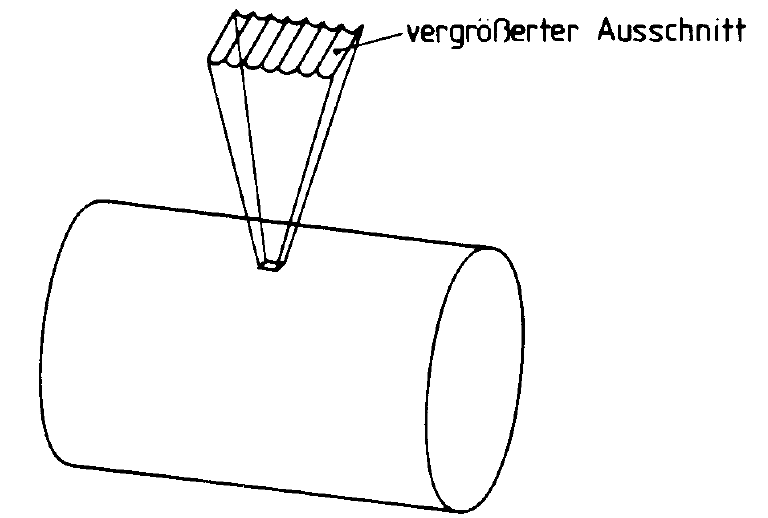
\includegraphics[width=0.5\linewidth]{img/DIN_4760_1}
	\caption[Ausschnitt aus der Istoberfläche zur Beurteilung der Gestaltabweichung]{Ausschnitt aus der Istoberfläche}
	\label{fig:din4760_1}
\end{figure}

Als Gestaltabweichungen 1.Ordnung werden in DIN 4760 jene Gestaltabweichungen beschrieben, die, wie weiter oben bereits angeschnitten, bei der Beurteilung der gesamten Istoberfläche ersichtlich werden. Abweichungen dieser Kategorie werden als Formabweichungen bezeichnet. Darunter zählen beispielsweise Geradheits- , Ebenheits- und Rundheitsabweichungen. Diese Art der Abweichungen begründet die Norm in fehlerhaften Führungen der bearbeitenden Maschine, Durchbiegung von Werkzeug oder Werkzeugmaschine, falscher Einspannung des Werkstückes, Verschleiß oder Härteverzug.

Die 2. Ordnung der Gestaltabweichungen wird unter dem Begriff Welligkeit geführt. Es handelt sich dabei um periodisch wiederholt auftretende Gestaltabweichungen der gemessenen Oberfläche eines untersuchten Formelements. Als wellig definiert die Norm DIN 4760 Abweichungen, bei denen das Verhältnis von Wellenabständen zur Wellentiefe generell zwischen 1000:1 und 100:1 liegt. Es handelt sich also um relativ niederfrequente Wellen mit einer verhältnismäßig niedrigen Amplitude. Als grundlegende Ursachen für die Entstehung von welligen Formen nennt die Norm sowohl außermittige Einspannung des Werkstücks als auch Form- und Laufabweichungen des Werkzeugs und Schwingungen der Werkzeugmaschine und des Werkzeugs.

Die Gestaltabweichungen 3. bis 5. Ordnung werden als Rauheit bezeichnet. Sie sind nur durch Betrachtung eines Oberflächenausschnitts des Objektes zu erkennen. Rauheitsabweichungen kehren entweder regelmäßig oder unregelmäßig wieder. Sie sind gekennzeichnet durch ein Verhältnis der Abstände zur Tiefe zwischen 100:1 und 5:1. Es handelt sich also im Vergleich zum im vorherigen Abschnitt beschriebenen Welligkeitsphänomen um hochfrequentere Abweichungen der Oberfläche. 
Innerhalb Klasse der Rauheitsabweichungen lassen sich veschiedene Ausprägungen beschreiben. So unterscheidet Rillen (4. Ordnung), Riefen, Schuppen, Kuppen (5.Ordnung) und Oberflächenrauheit, welche durch die Gefügestruktur hervorgerufen wird (6. Ordnung).
Diese Kategorien unterscheiden sich in Frequenz und Amplitude ihrer Form (siehe Abb. *Todo*). Außerdem lassen sich verschiedene Ursachen für ihr Auftreten finden. 

Rillen werden durch die Form der Werkzeugschneide sowie aufgrund des eingestellten Vorschubes und der Schnittbewegung des Werkzeuges hervorgerufen.
Riefen, Schuppen und Kuppen sind Oberflächenunvollkommenheiten, deren Gründe im Prozess der Spanbildung zu finden sind. Des Weiteren lassen sie sich beispielsweise durch Werkstoffverformung beim Strahlen oder Knospenbildung bei galvanischer Behandlung erklären. 

Rauheiten, welche durch die Gefügestruktur des Werkstoffes verursacht werden, sind durch Kristallisationsvorgänge oder Veränderungen der Oberfläche durch beispielsweise chemische oder korrosive Vorgänge entstanden. Sie bilden zusammen mit der 6. Ordnung der Gestaltabweichungen, welche durch den Gitteraufbau des Materials zu erklären sind, die nicht mehr durch Messverfahren ermittelbaren Gestaltabweichungen. 

Das bedeutet, dass in der Istoberfläche für gewöhnlich eine Struktur zu erkennen ist, die durch Überlagerung der Gestaltabweichungen 1. bis 4. Ordnung verursacht wird. 

\subsubsection{Oberflächenunvollkommenheiten}

Zusätzlich zu den in DIN 4760 aufgeführten Gestaltabweichungen werden in DIN EN ISO 8785 Oberflächenunvollkommenheiten erläutert. In der Norm werden diese als "`Element, Unregelmäßigkeit oder Gruppe von Elementen und Unregelmäßigkeiten der wirklichen Oberfläche, die unbeabsichtigt oder zufällig durch die Bearbeitung, Lagerung oder Funktion der Oberfläche entstanden sind"' definiert. Es wird dabei unterschieden zwischen nach innen orientierten (Vertiefung), nach außen gerichteten (Buckel), kombinierten und stellenweisen Oberflächenunvollkommenheiten. Kombinierte Oberflächenunvollkommenheiten enthalten sowohl Anteile von Vertiefungen als auch Buckeln. Stellenweise Unvollkommenheiten besitzen eine kaum messbare Erhöhung bzw. Vertiefung. 

In \prettyref{fig:din-en-8785-beispiele} sind einige Beispiele für jede genannte Kategorie der Oberflächenunvollkommenheiten zu finden. 

\begin{figure}[h]
	\centering
	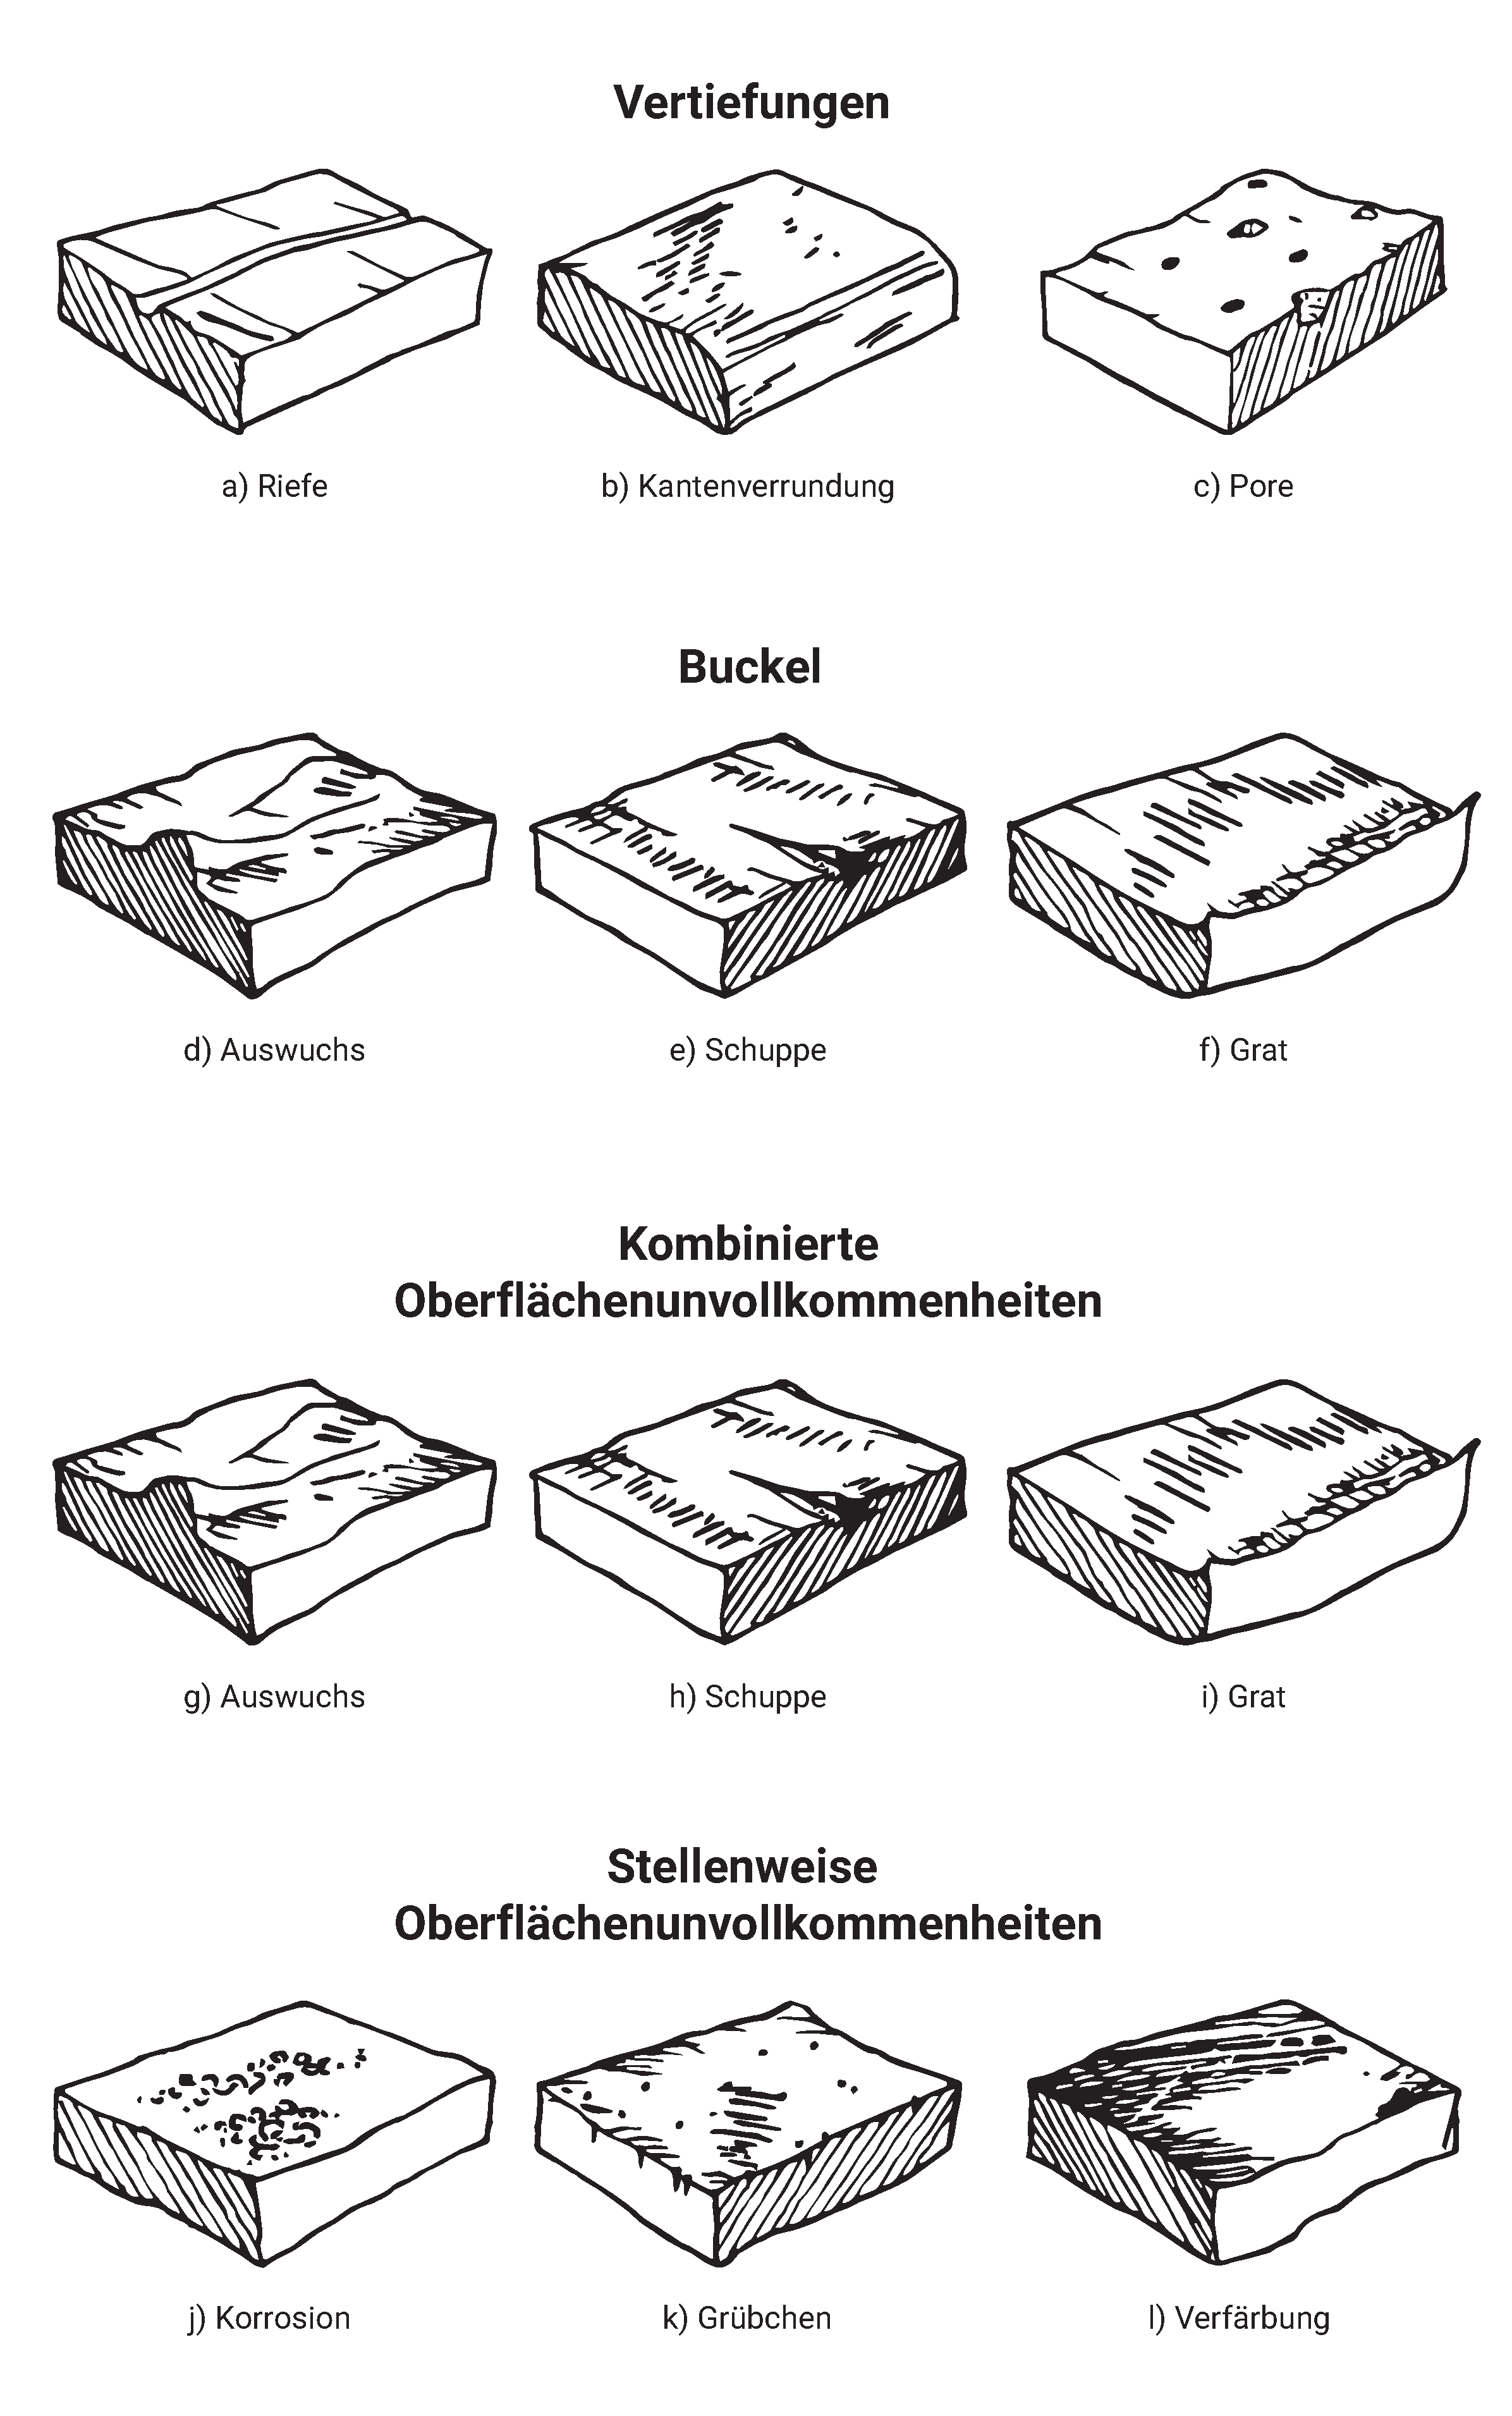
\includegraphics[width=0.7\linewidth]{img/din_en_8785_beispiele}
	\caption[DIN EN 8785 - Oberflächenunvollkommenheiten]{DIN EN 8785 - Oberflächenunvollkommenheiten}
	\label{fig:din-en-8785-beispiele}
\end{figure}









 






          


